\chapter{Lecture 25 - Solving IVPs with Runge-Kutta Methods}
\label{ch:lec25n}
\section{Objectives}
The objectives of this lecture are to:
\begin{itemize}
\item Qualitatively motivate and describe the derivation of Runge-Kutta methods
\item Do some example problems
\end{itemize}
\setcounter{lstannotation}{0}

\section{Runge-Kutta Methods}
Runge-Kutta (RK) methods are a family of single-step numerical methods for solving first order initial value problems.
\begin{align*}
y^{\prime} &= f(t,y) \\
y(0) &= y_0
\end{align*}
The basic idea stems from that of Euler's methods where we approximated $y_{n+1}$ based on $y_n$, the slope, $y^{\prime}=f(t,y)$, and the step size.
\begin{equation*}
y_{n+1} = y_n + f(t,y)h
\end{equation*}
This can be expressed more exactly in terms of integrals:
\begin{equation*}
y_{n+1}=y_n+\int y^{\prime} \ \text{dt} = y_n+\int_{t_{n}}^{t_{n+1}} \ f(t) \ \text{dt}
\end{equation*}
In your earlier classes in ordinary differential equations, this is a standard solution method for separable initial value problems:
\begin{equation*}
\frac{dy}{dt} = y^{\prime} = \frac{h(t)}{g(y)} \Rightarrow \int g(y) \ \text{dy} = \int h(t0 \ \text{dt}
\end{equation*}
For the simple case where $g(y) = 1$ and we integrate over one time step we get:
\begin{equation*}
\int_{y_{n}}^{y_{n+1}} 1 \ \text{dy} \rightarrow y_{n+1} = y_n + \int_{t_n}^{t_{n+1}} f(t)\ \text{dt}
\end{equation*}
Let us generalize a bit further and consider first order IVPs in the form:
\begin{equation}
y_{n+1} = y_n + \int_{t_n}^{t_{n+1}} f(t,y) \ \text{dt}
\label{eq:lec25n-1}
\end{equation}
and propose that we use \emph{quadrature} instead of exact integration.  Now we can re-write Equation \ref{eq:lec25n-1} as:\marginnote{\textbf{Note:} With this notation, $y_n = y(t_n)$ and $y_{n+1} = y(t_{n+1})$.}
\begin{equation}
y_{n+1} = y_n + h \sum\limits_{i=1}^{s} b_i f(t_n + c_ih,y(t_n+c_ih))
\end{equation}
where $h$ is like the scaling term, $\sfrac{b-a}{2}$, in Gauss quadrature, $b_i$ are the weights, and $c_i$ are the sample points.  We constrain $c_i \in [0,1]$ so that $t_n \le (t_n+c_ih) \le t_{n+1}$. \marginnote[-0.5cm]{\textbf{Note:} To prevent confusion with Guass quadrature, from now on, we will refer to $c_i$ as the \emph{RK nodes} and $b_i$ as the \emph{RK weights}.}

\newthought{One problem with} this approach is that we do not know the values: $y(t_n+c_jh)$.  In RK methods, we will approximate these points between $y_n$ and $y_{n+1}$ as follows:
\begin{align*}
\xi_{\nu} &= y_n + h\sum\limits_{i=1}^{s}a_{\nu,i}f(t_n+c_ih,\xi_i) \\
y_{n+1} &= y_n + h\sum\limits_{i=1}^{s}b_i f(t_n+c_ih,\xi_i)
\end{align*}
The number of sample points, $s$, is referred to as the number of \emph{stages} and the elements $a_{\nu,i}$ are customarily arranged into a square matrix, called the \emph{RK matrix}.  As an example, for a 2-stage system, we can write out these equations fully as:\marginnote[0.75cm]{\textbf{Note:} Notice that the top equation is, in general, non-linear and must be solved iteratively using one of the methods we learned for non-linear systems of equations.  If the RK matrix is strictly lower triangular---i.e. only non-zero below the main diagonal---then the values for $\xi_i$ can be solved without iteration.}
\begin{align*}
\bracketVectorstack{\xi_1 \\ \xi_{2}} &= y_n + h\bracketMatrixstack{a_{11} & a_{12} \\ a_{21} & a_{22}} \bracketVectorstack{f(t_n+c_1h,\xi_1) \\ f(t_n+c_2h,\xi_2)} \\
y_{n+1} &= y_n + h \bracketMatrixstack{b_1 & b_2}\bracketVectorstack{f(t_n+c_1h_1,\xi_1) \\ f(t_n+c_2h,\xi_2)}
\end{align*}
\begin{marginfigure}
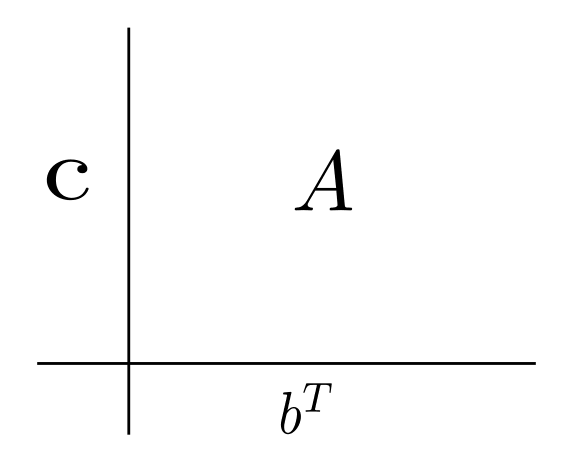
\includegraphics{lec25n-butcher-tableau.png}
\caption{Schematic of a Butcher Tableau.}
\label{fig:lec25n-butcher-tableau}
\end{marginfigure}
For an \emph{explicit} RK method, the RK matrix is strictly lower triangular.  The values of the RK weights, RK nodes, and entries in the RK matrix are customarily organized as a Butcher Tableau\cite{butcher2016numerical} as illustrated in Figure \ref{fig:lec25n-butcher-tableau}.  

In this class we will not derive any RK methods from scratch.  Still, we can make some general observations about RK methods:
\begin{enumerate}
\item The order of convergence for explicit RK methods is equal to the number of stages, for $s<=4$.  RK methods with greater than 4\textsuperscript{th}-order convergence have been derived, but in those cases the number of stages, $s$, is greater than the order of convergence.

\item The sum of each row in the RK matrix is equal to the corresponding RK node.
\item the sum of the RK weights is equal to 1.
\end{enumerate}

\newthought{From this perspective} the modified Euler's method presented in the last lecture is equivalent to a 2-stage RK method. The RK nodes, RK weights, and RK matrix are shown below:
\begin{equation*}
c = \bracketVectorstack{0 \\ 1}, \ \ b^{T} = \bracketMatrixstack{\sfrac{1}{2} & \sfrac{1}{2}}, \ \ A = \bracketMatrixstack{0 & 0 \\ 1 & 0}
\end{equation*}
and the Butcher Tableau is shown in Table \ref{tab:lec25n-mem-tableau}.
\begin{margintable}
\begin{tabular}{c|cc}
0 & 0 & 0 \\
1 & 1 & 0 \\ \hline
  & $\sfrac{1}{2}$ & $\sfrac{1}{2}$ \\
\end{tabular}
\caption{Butcher Tableau for the modified Euler's method.}
\label{tab:lec25n-mem-tableau}
\end{margintable}

\section{MATLAB Implementation of RK Methods}

In this section I will present and explain three successive MATLAB implementations of an RK method.  The goal for this implementation is clarity and generality, not performance.  Students who are interested in achieving greater performance are encouraged to find optimizations sometime \emph{after} they fully understand what is shown here.

\subsection{2\textsuperscript{nd}-Order RK Method, Scalar 1\textsuperscript{st}-Order Equation}
We will start with an implementation of the modified Euler's method cast as an RK method for a scalar differential equation of 1\textsuperscript{st}-order.  The first portion of the function is shown in the listing below. Here we document the input and output variables; define variables to hold the RK matrix, RK weights, and RK nodes; and allocate a vector for the solution.

\begin{lstlisting}[style=myMatlab,name=lec25n-1]
function y = odeRK2(f,a,b,N,yINI)
% function y = odeRK2(f,a,b,h,yINI)
% y = solution
% f = function handle for y'
% a,b = interval for solution
% N = number of steps between a and b (inclusive)
% yINI = initial value for the solution

A = [0 0;
    1 0]; % RK matrix
B = [0.5 0.5]; % weights
c = [0 1]';% sample points
stages = 2;

x = linspace(a,b,N);
y = nan(1,N);
y(1) = yINI;
h = x(2)-x(1);
\end{lstlisting}

\noindent Now we will calculate RK solution process:\marginnote{

\vspace{0.5cm}

\noindent\ref{lst:ann25n-1} A new array of slopes, one element for each stage, will ne needed at each time step.

\vspace{0.3cm}

\noindent\ref{lst:ann25n-2} This nested for loop calculates:
$$\xi_{s} = y_n + h\sum\limits_{i=1}^{s-1} a_{s,i}f(t_n+c_ih,\xi_{i})$$
for each value of $s$.  The upper limit of the summation index,$s-1$, is due to the fact that this is an explicit method and the RK matrix is strictly lower triangular.

\vspace{0.2cm}

\noindent\ref{lst:ann25n-3} This loop calculates:
$$y_{n+1} = y_n + h\sum\limits_{i=1}^{s}b_if(t_n+c_ih,\xi_i)$$

}
\begin{lstlisting}[style=myMatlab,name=lec25n-1]
for t = 1:(N-1)
    Xi = nan(1,stages); /*!\annotation{lst:ann25n-1}!*/
    
    for s = 1:stages
       Xi(s) = y(t); /*!\annotation{lst:ann25n-2}!*/
       for i = 1:(s-1)
          Xi(s) = Xi(s) + ...
              h*A(s,i)*f(x(t)+c(i)*h,Xi(i)); 
       end
    end
    
    y(t+1) = y(t);
    for i = 1:stages
       y(t+1) = y(t+1) + ...
           h*B(i)*f(x(t)+c(i)*h,Xi(i)); /*!\annotation{lst:ann25n-3}!*/
    end    
end
end
\end{lstlisting}






